\chapter{Programa de Visualização}\label{cap:swpc}

		Dentre os requisitos listados na seção \ref{lst:swpc:req}, o controle de transferência de dados e apresentação de informações de estado são apresentados nas seções \ref{sec:swpc:flow} e \ref{sec:swpc:gui:stats}, respectivamente. Assim como um osciloscópio, o programa deverá oferecer a opção de apresentação de dados de forma contínua ou por amostragem. Detalhes sobre este recurso são apresentados na seção \ref{sec:swpc:gui:graph}. A exportação de dados nos formatos binário e CSV são comuns entre os instrumentos de medição, determinando assim que o programa seja compatível com estes formatos. Da mesma forma, a captura de imagens em formato em .png e .jpg é necessário. Os processos de exportação de dados e captura são detalhados na seção \ref{sec:swpc:save}.
		\index{.jpg}
		\index{.png}
		\index{CSV}
		\index{.bin}

		O programa foi desenvolvido em C\# no IDE Microsoft Visual Studio Community\textsuperscript{\textregistered}. A comunicação com sistema de controle e a geração de elementos gráficos foi implementada com os recursos da plataforma .NET.
		\index{.NET}
		\index{C\#}
		\index{Microsoft Visual Studio Community \textsuperscript{\textregistered}}

		O código fonte do programa está presente nos Apêndices \ref{app:source:mygrapher}, em que as variáveis, funções e métodos são declarados e utilizados, e \ref{app:source:gui}, o qual contém as definições da interface gráfica.
		\index{IG}

	\section{Interface Gráfica de Usuário}\label{sec:swpc:gui}

		O principal objetivo da IG é a fácil apresentação dos dados enviados pelo escravo. Isto é alcançado pela maximização da área ocupada pelo gráfico, existência de poucos parâmetros de configuração e codificação do estado de operação por cores. A área visível da IG pode ser dividida em quatro seções: Estatística e Estado, Gráfico, Início e Pausa e Configuração. Estas seções são dispostas conforme apresentado na Figura \ref{img:swpc:screenshot}.

		\begin{figure}[h]
			\caption{Programa de aquisição e apresentação de dados}
			\label{img:swpc:screenshot}
			\begin{tikzpicture}[rounded corners=0.1cm, opacity=0.72, shorten >=0.2cm]
			%\draw[help lines, step=0.5] (0, 0) grid (15,10);
			\node (img) [inner sep=0pt, outer sep=0pt] at (0.5*\textwidth,5) {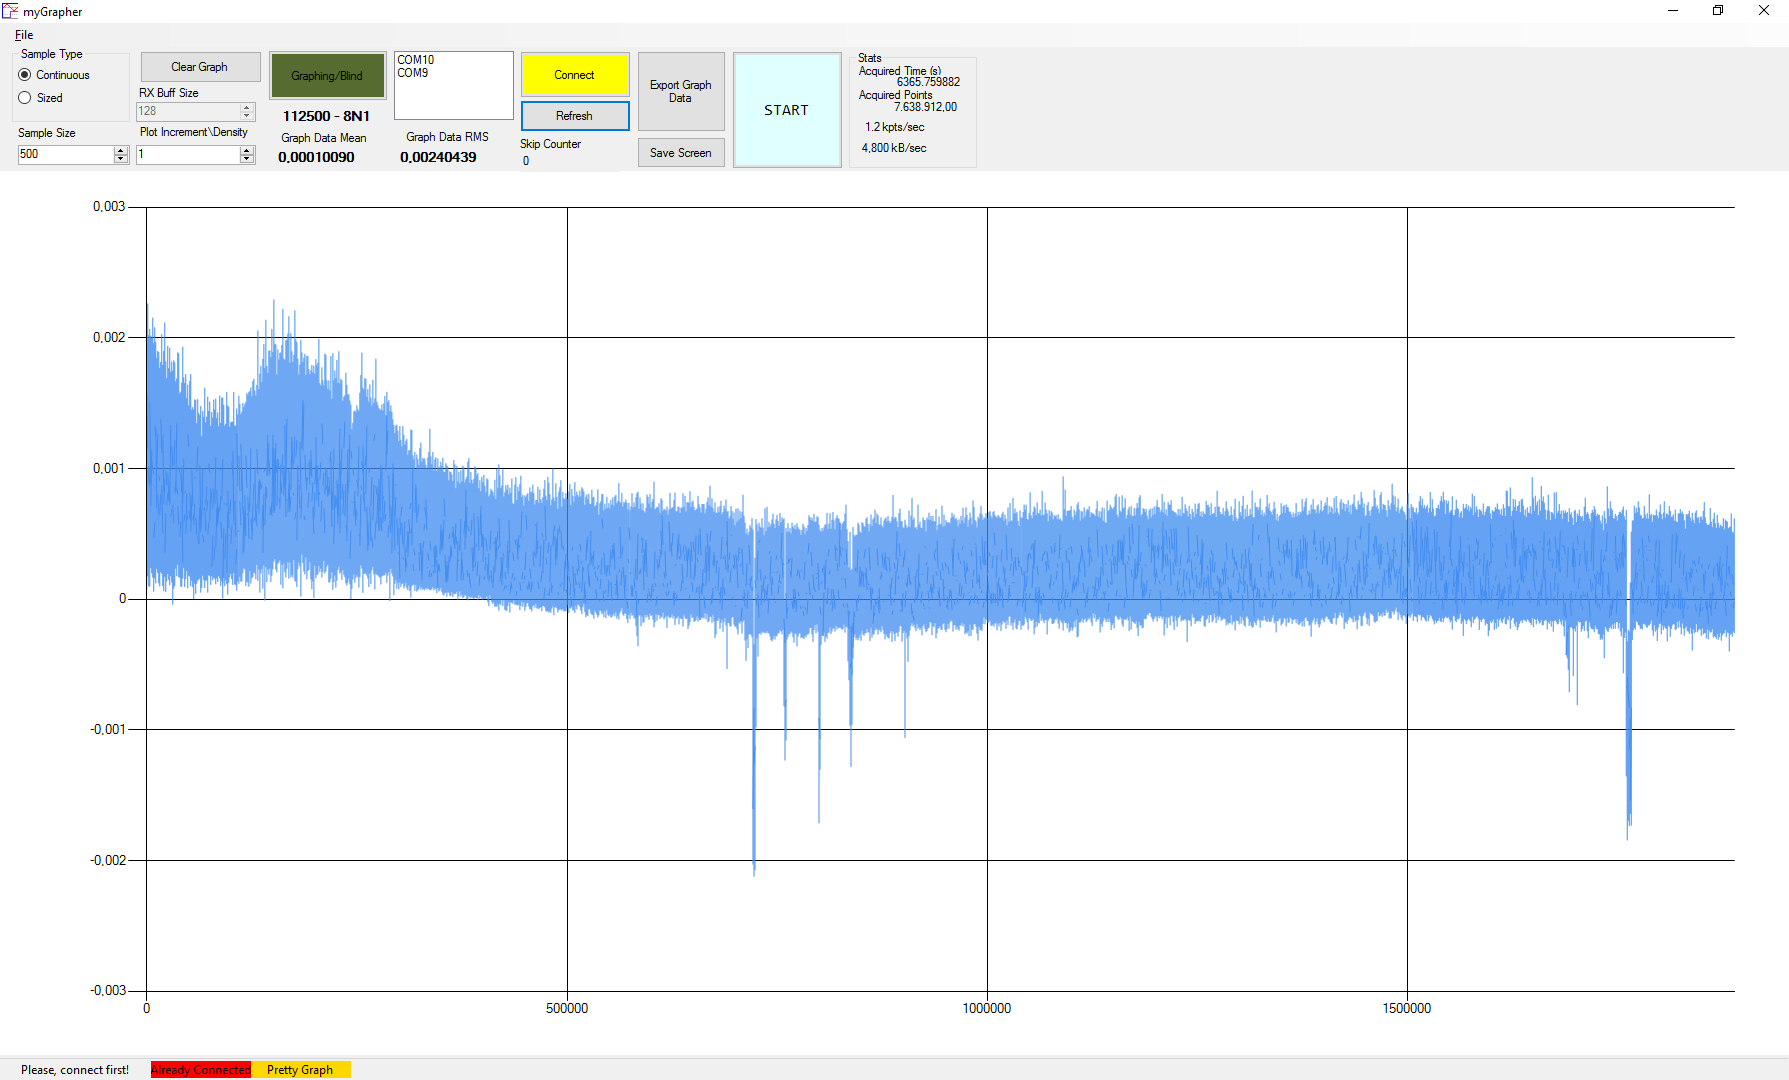
\includegraphics[width=\textwidth,center]{images/appinaqcuisitionmode}};
			\node (graph) at (14, 11) {Gráfico};
			\node (qgraph) at (8.5,4.375) [rectangle, fill=lightgray!45, minimum width=0.96*\textwidth, minimum height=7.6cm] {};
			
			\node (config) at (2,11) {Configuração};
			\node (qconfig)at (3.25, 8.85) [rectangle, fill=olive!45, minimum width=6.5cm, minimum height=1.25cm] {};
			
			\node (inicio) at (5.5,11) {Início e Pausa};
			\node (qinicio) at (7.1, 8.85) [rectangle, fill=teal!45, minimum width=1.2cm, minimum height=1.25cm] {};
			
			\node (stats) at (10,11) {Estatística e Estado};
			\node (qstats) at (8.25, 8.85) [rectangle, fill=brown!45, minimum width=1.2cm, minimum height=1.25cm] {};
			\node (botstats) at (1.75, 0.25) [rectangle, fill=brown!45, minimum width=3.5cm, minimum height=0.3cm] {};
			
			\draw[thick, ->] (config) to [out=270, in=90] (qconfig);
			\draw[thick, ->] (inicio) to [out=270, in=90] (qinicio);
			\draw[thick, ->] (stats.south)  to [out=270, in=90] (qstats);
			\draw[thick, ->] (stats.south)  .. controls +(0,-10) and +(0,4) .. (botstats.north);
			\draw[thick, ->] (graph)  to [out=270, in=90] ($(qgraph.north east) +(-1,0)$);
			\end{tikzpicture}
		\end{figure}

		\subsection{Estatística e Pausa}\label{sec:swpc:gui:stats}

			Esta seção apresenta informações de número de pontos recebidos, quantidade de dados (em kB), tempo de aquisição, e médias de velocidade sobre a última transferência de dados realizada. O número de pontos e a quantidade de dados estão relacionados diretamente pelo tamanho que cada ponto ocupa. No caso da codificação em números flutuantes de 32 bits (\textit{single precision float}), cada ponto apresenta um tamanho de 4 bytes. A média de pontos por segundo e taxa de transferência são calculadas a partir do número total de pontos adquiridos e o tempo de recepção. A área no rodapé da janela do programa apresenta algumas informações sobre a configuração de alguns parâmetros descritos na \ref{sec:swpc:gui:config}.
			\index{float}
			\index{Número Flutuante}

			% ADD na seção do CDC que o protocolo necessita da trasnferência do ACK para transmissão de outro quadro, forçando assim a correta ordenação dos dados

		\subsection{Gráfico}\label{sec:swpc:gui:graph}

			Esta seção apresenta em forma de gráfico $XY$ os pontos recebidos por meio de dois métodos: Contínuo e por amostragem. Em ambos os métodos o eixo $Y$ apresenta os valores recebidos sem alteração ou aplicação de escalas, enquanto o eixo $X$ apresenta o número de amostras apresentadas.
			\iffalse No método contínuo, os valores no eixo $X$ são incrementados na taxa de $(Pontos/s)/n$, enquanto que no método por amostragem o eixo $X$ é constante e determinado por \textit{Sample Size}.\fi % UNCUT

			O método contínuo apresenta os pontos de forma incremental, ou seja, mantém os pontos presentes no gráfico e adiciona os novos pontos recebidos. Devido a esta característica o número de pontos presentes no gráfico sempre irá ser acrescido. Este método é útil para a visualização de variações ao longo do tempo e a posterior realização de comparações visuais. Em um cenário ideal todos os pontos recebidos são apresentados no gráfico. Entretanto a operação com altas taxas de transferência requer uma maior capacidade de processamento para a atualização do gráfico. A construção atual do programa é baseada em bibliotecas com um alto nível de abstração e complexidade, impossibilitando a adição de todos os pontos no gráfico durante altas taxas de transferência. Para contornar esta particularidade, o parâmetro \textit{Plot Increment} foi criado. Este é uma variável no programa do tipo inteiro (e maior que 0), e determina uma relação entre o número de pontos salvos na memória e o número de pontos presentes no gráfico. A interpretação da influência deste parâmetro no programa é: ``$1$ ponto a cada $n$ pontos recebidos será adicionado ao gráfico.''
			\index{Plot Increment}
			\index{Atualiza Gráfico}

			O método por amostragem, por outro lado, possui um número fixo de pontos apresentados que são substituídos a cada atualização. Este número de pontos é determinado pelo parâmetro \textit{Sample Size}. O parâmetro \textit{Plot Increment} também é utilizado neste método, porém apresentando outra interpretação. Ao considerar que os dados recebidos são correspondentes a valores adquiridos em intervalos iguais, é possível afirmar que \textit{Plot Increment} multiplica em $n$ vezes a escala temporal do gráfico.
			\index{Sample Size}
			\index{Atualiza Gráfico}



		\subsection{Início e Pausa}\label{sec:swpc:gui:start}

			Esta seção consiste apenas no botão que habilita ou desabilita a recepção de dados e atualização do gráfico, através do sinal DTR.
			\index{DTR}
			\index{Atualiza Gráfico}

		\subsection{Configuração}\label{sec:swpc:gui:config}

			Esta seção apresenta botões para controle de configuração e parâmetros de programa que podem ser modificados pelo usuário. Os parâmetros, na forma ``\textbf{nome do parâmetro / variável} Descrição (\textbf{valor inicial}/outros valores válidos),'' são:

			\begin{samepage}
				\begin{description}
					\item[\textit{sampleContinuous}] Método de apresentação no gráfico (\textbf{contínuo} / por amostragem);
					\item[\textit{sampledSize}] Número de pontos apresentados no método por amostragem (\textbf{500}, valor mínimo: 10);
					\item[\textit{plotIncrement}] Valor de incremento na varredura da memória (\textbf{128}, 1-8192);
					\item[\textit{buffSize}] Tamanho, em bytes, do buffer de recepção (\textbf{128} -  8192);
					\item[\textit{graphEn}] Habilita ou suprime a atualização dos dados no gráfico, ativado pelo botão \textit{Graphing / Blind} (\textbf{ativo} / inativo);
					\item[\textit{serialPort1} \& \textit{portsListBox}] Nome da porta serial selecionada / ativa (\textbf{sem seleção});
					\item[\textit{sysConnected}] Estado de conexão programa com porta serial, ativado pelo botão \textit{Connect} (\textbf{desconectado} / conectado);
					\item[\textit{receiveIsActive}] Estado de habilitação da recepção de dados, ativado pelo botão \textit{START} (\textbf{desabilitado} / \textbf{habilitado}).
				\end{description}
			\end{samepage}
			\index{sampleContinuous}
			\index{sampledSize}
			\index{plotIncrement}
			\index{buffSize}
			\index{graphEn}
			\index{serialPort1}
			\index{sysConnected}
			\index{receiveIsActive}
			\index{Graphing}
			\index{Blind}
			\index{START}
			\index{serialPort1}
			\index{portsListBox}

			Os botões de controle, na forma ``\textbf{nome do botão} Descrição da ação,'' são:

			\begin{description}
				\item[\textit{Clear Graph}] Limpa os dados armazenados na memória e apresentados no gráfico;
				\item[\textit{Refresh}] Atualiza a lista de portas seriais disponíveis no computador;
				\item[\textit{Export Graph Data}] Abre caixa de diálogo para exportação dos dados recebidos e armazenados;
				\item[\textit{Save Screen}] Abre caixa de diálogo para captura da imagem do programa.
			\end{description}
			\index{Clear Graph}
			\index{Refresh Ports}
			\index{Export Graph Data}
			\index{Save Screen}


	\section{Estados de Operação}\label{sec:swpc:flow}

			O programa apresenta quatro estados de operação, sendo um destes intermediário, conforme apresentado no diagrama da Figura \ref{img:swpc:modos}. O programa é inicializado no estado Espera, a troca de estado para Configuração ocorre quando o usuário realiza a conexão com a porta serial. Nesta mudança o valor da variável \textit{sysConnected} é alterado para verdadeiro. Da mesma forma, a subsequente troca de estado para Aquisição ocorre quando o usuário habilita a recepção de dados pelo parâmetro \textit{receiveIsActive}.
			\index{sysConnected}
			\index{receiveIsActive}

			A transição para o estado intermediário ocorre a partir dos estados de Espera e Configuração. A transição é ativada pelo usuário utilizando o botão correspondente na IG. Após a exportação dos dados, o programa retorna ao estado anterior, sem modificações nas configurações salvas. Durante o processo de exportação dos dados, a área de Estatística e Pausa de rodapé notifica o início e término da operação.
			\index{IG}

			\begin{figure}[h]
			\caption{Estados de operação do programa}
			\label{img:swpc:modos}
			\centering
			\begin{tikzpicture}[block diagram, node distance=2.5cm]
				\node (inout)	[text label]								{};
				\node (wait)	[blue block, right =56pt of inout]			{Espera};
				\node (exp)		[blue block, below =of wait]				{Exportação\\de Dados};
				\node (config)	[blue block, right =of wait]				{Configuração};
				\node (acq)		[blue block, above right =of config]		{Aquisição};

				\draw [thick, ->]	(config)		to [bend right=45]		node [below right, text label] 	{DTR = 1}			(acq);
				\draw [thick, ->]	(acq)			to [bend right=15]		node [above left, text label] {DTR = 0}	(config);
				\draw [thick, ->]	(wait)		--		node [below, text label] 			{Sistema\\Conectado}		(config);
				\draw [thick, ->]	(config)	.. controls +(-2.15,2.15)..		(wait);
				\draw [thick, ->]	(acq)		.. controls +(left:5cm)..	node [above, text label]			 {Desconectar}				(wait);
				\draw [thick, <->]	(wait)			--		node [below, text label]	{Entrada\\Saída}										(inout);
				\draw [thick, <->]		(wait)		--		node [right, yshift=-0.5cm, text label]	{Botão\\Exportar}		(exp);
				\draw [thick, <->]		(config)	to [bend left=45]	node [below, xshift=1cm, text label]	{Botão\\Exportar}				(exp);
			\end{tikzpicture}
			\end{figure}

			Os estados da Figura \ref{img:swpc:modos} podem ser separados de acordo com a sua combinação de variáveis \textit{sysConnected} e \textit{receiveIsActive}, de acordo com o Quadro \ref{tab:swpc:stateschange}. O estado Exportação de Dados não altera o valor da variável \textit{sysConnected} durante sua execução, voltando portando ao estado anterior a sua chamada.
			\index{sysConnected}
			\index{receiveIsActive}


			\begin{table}
				\caption{Relação entre estados do programa e variáveis de estado}
				\label{tab:swpc:stateschange}
				\centering
				\begin{tabular}{|c|c|c|}
					\hline
					\textbf{Estado}	&	\textbf{sysConnected}	&	\textbf{receiveIsActive}		\\ 	\hline
					Espera			&	0						&	0								\\	\hline
					Configuração	&	1						&	0								\\	\hline
					Aquisição		&	1						&	1								\\	\hline
					Exportação de Dados	&	X					&	0								\\ 	\hline
				\end{tabular}
			\end{table}


		\subsection{Espera}\label{sec:swpc:wait}

			Neste estado o programa não realiza atividades ou cálculos. A condição para a transição de estado é a seleção de uma porta serial válida. A transição deste estado para Configuração é ativada pelo usuário, através do botão \textit{Connect} e pela função \textit{private void \textbf{connectClick}(object sender, System.EventArgs e)}. Esta função atualiza os tamanhos dos \textit{buffers} da porta serial e os indicadores de estado do programa. Neste estado todos as opções da IG podem ser modificadas, assim que todos os parâmetros podem ser escolhidos e configurados anteriormente ao início de funcionamento do programa.
			\index{IG}
			\index{connectClick}

		\subsection{Configuração}\label{sec:swpc:config}

			Neste estado somente os parâmetros \textit{sampleContinuous}, \textit{sampledSize}, \textit{plotIncrement} e \textit{graphEn} podem ser modificados. As opções de escolha de porta serial e tamanho do \textit{buffer} de entrada estão desabilitadas.
			\index{sampleContinuous}
			\index{sampledSize}
			\index{plotIncrement}
			\index{graphEn}

			No retorno do estado Aquisição a área de Estatísticas é atualizada.


		\subsection{Aquisição}\label{sec:swpc:acq}

			A Figura \ref{img:swpc:dataflow:run} apresenta o diagrama de fluxo de dados no programa durante o estado de aquisição. Este diagrama apresenta três caminhos distintos: caminho ativo (\tikz[baseline=-3pt] \draw [draw, thick, ->] (0,0) -- (24pt,0);), caminho inativo (\tikz[baseline=-3pt] \draw [draw, dashed, blue, ->] (0,0) -- (24pt,0);) e caminho independente (\tikz[baseline=-3pt] \draw [draw, dotted, ->] (0,0) -- (24pt,0);). O bloco ``RxIRQ'' realiza a recepção e sincronia dos dados recebidos, os bancos \textit{bank0} e ``bank1'' são ``buffers'' intermediários, o bloco ``Atualiza Gráfico'' realiza o procedimento de atualização do gráfico apresentado ao usuário e por fim o bloco ``mainMem'' representa a memória principal do programa.
			\index{RxIRQ}
			\index{bank0}
			\index{bank1}
			\index{mainMem}

			O bloco ``RxIRQ'' é implementado na função \textit{private void \textbf{receiveContinuous}(Object o, EventArgs e)} do tipo \textit{callback}. Esta é executada quando o nível de utilização do \textit{buffer} de entrada da porta serial atingir \nicefrac{2}{6}. Este valor relativamente baixo foi determinado para garantir a contínua recepção de dados, evitando a perda por falta de espaço para recepção. A capacidade total é definida como seis vezes o tamanho definido pelo usuário no controle correspondente na IG. Estas duas configurações são realizadas na função \textit{private void \textbf{updatePointsSize}(Int32 size)}, executada toda vez que o usuário realiza a conexão serial com o \textit{hardware}. A execução de ``RxIRQ'' resulta na cópia dos dados recebidos desta função para o \textit{buffer} intermediário ativo, \textit{bank0} ou \textit{bank1}. Na versão atual, o programa armazena os dados recebidos de forma sequencial sem informação temporal.
			\index{RxIRQ}
			\index{receiveContinuous}
			\index{callback}
			\index{updatePointsSize}
			\index{bank0}
			\index{bank1}

			Os \textit{buffers} intermediários possuem tamanho fixo de $6 \cdot 4096$ bytes cada, resultando em $6 \cdot 1024$ pontos, e são responsáveis pela sincronização da recepção de dados e escrita na memória principal. Enquanto um \textit{buffer} recebe os dados de ``RxIRQ'' o outro transfere seu conteúdo para ``mainMem''. Após esta transferência o procedimento de atualização do gráfico é realizado. Esta etapa é realizada de forma assíncrona à recepção e tratamento dos dados, garantindo nenhuma interrupção ou perda.
			\index{mainMem}
			\index{Atualiza Gráfico}

			A memória principal, ``mainMem'', é paginada com tamanho máximo de 32 milhões de pontos para aquisição, ocupando 128 MB de memória dinâmica. A utilização das páginas de ``mainMem'' é realizada conforme necessário, sendo estas criadas por alocação dinâmica durante a execução do programa.
			\index{mainMem}

			\begin{figure}[h]
				\caption{Fluxo de dados durante aquisição}
				\label{img:swpc:dataflow:run}
				\begin{tikzpicture}[block diagram, every rectangle node/.append style={blue color}]
				%picture centered at rx irq block
				%\draw[help lines] (0,-10) grid (16,10);
				%\node (block) at (8,0) [draw, rectangle, minimum width=16cm, minimum height=8cm] {};
				%\draw [draw, thick] (0,-4) rectangle (16,8);
				\node (rxirq) at +(4.5,0)	[draw, thick, rectangle, minimum width=1.5cm,  minimum height=2cm, align=center] {Rx\\IRQ};
				\node (bank0) at +(8,+0.75)	[draw, thick, rectangle, minimum width=2cm,  minimum height=1.5cm, align=center] {bank0};
				\node (bank1) at +(8,-0.75)	[draw, thick, rectangle, minimum width=2cm,  minimum height=1.5cm, align=center] {bank1};
				\node (refresh) at +(14, 0) [draw, thick, rectangle, minimum width=4cm, minimum height=2cm, align=center] {Atualiza\\Gráfico};

				\node (mem)   at +(9,6) [draw, thick, rectangle, minimum width=12cm, minimum height=1cm, align=center, inner sep=0pt, outer sep=0pt] {mainMem};
				\foreach \x in {0,...,9}
					\node (pg\x) at ($ (mem.south west) + (\x +0.5, -0.5) $) [draw, thick, rectangle, minimum width=1cm, minimum height=1cm, align=center] {$\x$};
				\node (pgdot) at ($ (mem.south west) + (10 +0.5, -0.5) $) [draw, thick, rectangle, minimum width=1cm, minimum height=1cm, align=center] {\dots};
				\node (pgn) at ($ (mem.south west) + (11 +0.5, -0.5) $) [draw, thick, rectangle, minimum width=1cm, minimum height=1cm, align=center] {$n$};
	%	\draw [arrow]	(switch) -- node[anchor=south, xshift=0.5cm]{Atualiza Gráfico} node[anchor=north]{(a)}		(flag);

				\draw [draw, thick, ->]				($ (rxirq.west) + (-2,0) $)		--	node[text label, above, align=center] {Conexão\\com\\Hardware}				(rxirq.west);
				\draw [draw, dotted, ->]			(pg8.south)					to [out=270, in=90]		(refresh.north);		% before to keep it lower
				\draw [draw, ->, blue, dashed]		(rxirq.east)				to [out=0, in=180]		(bank1.west);			% before to keep it lower
				\draw [draw, thick, ->] 			(rxirq.east)				to [out=0, in=180]		(bank0.west);
				\draw [draw, ->, blue, dashed]		(bank0.east)				to [out=0, in=270]		(pg9.south);
	%			\draw [draw, ->, blue, dashed]		(bank1.east)				to [out=0, in=270]		(pg9.south);
				\draw [draw, thick, ->]				(bank1.east)				to [out=0, in=270]		(pg8.south);	% last to keep it higher

				%legend
				\draw [draw, dotted, ->]			($(rxirq.north) + (-1,1)$)		--				($(rxirq.north) + (1,1)$)	node [text label, align=left, xshift=1.3cm]{Facultativo};
				\draw [draw, ->, blue, dashed]		($(rxirq.north) + (-1,1.5)$)	--					($(rxirq.north) + (1,1.5)$) 	node [text label, align=left, xshift=1cm]{Inativo};
				\draw [draw, thick, ->]				($(rxirq.north) + (-1,2)$)		--				($(rxirq.north) + (1,2)$)	node [text label, align=left, xshift=1cm]{Ativo};

				\end{tikzpicture}
			\end{figure}
			\index{bank0}
			\index{RxIRQ}
			\index{bank1}
			\index{mainMem}
			\index{Atualiza Gráfico}

			O controle do fluxo e a cópia dos dados são gerenciadas pelo mesmo programa, sendo necessária a utilização de funções \textit{callback}, ferramentas de sincronização e múltiplas \textit{threads} para atender os prazos de execução. A plataforma .NET possui a classe \textit{BackgroundWorker}, a qual implementa uma forma de ativação de procedimentos concorrentes, chamados \textit{DoWork}. Esta classe também possui a opção de execução de um terceiro procedimento, ativado após o término de \textit{DoWork}. Esta classe foi utilizada para a implementação das funções de cópia dos bancos intermediários para a memória e para a atualização do gráfico.
			\index{BackgroundWorker}
			\index{callback}
			\index{DoWork}
			\index{threads}
			\index{.NET} 

			O digrama da Figura \ref{img:swpc:schedule} apresenta a organização temporal dos procedimentos execução durante o início de \textit{DoWork}. O gráfico de ``Processamento Resultante'' apresenta uma estimativa da organização do tempo utilizado pelo programa considerando um processador de núcleo individual e sem suporte a múltiplas \textit{threads}. O tempo de processador gasto em outras \textit{threads}, tarefas ou com o sistema operacional não é considerado.
			\index{threads}
			\index{DoWork}

			\begin{figure}[h]
				\caption{Diagrama temporal de execução de tarefas do programa}
				\label{img:swpc:schedule}
				\centering
				\begin{tikzpicture}[indi/.style={->, thick, black, shorten >=8pt, shorten <=8pt}]
				\foreach \x in {0,...,11}
					\draw [draw,ultra thin, gray!30] (\x, 0) -- (\x, -8);
				%start graph lines
				\draw [thick, <->]	(0,0) node 	[anchor=west, yshift=-1.2cm, xshift=-2cm] {RxIrq}	--	(0,-2)	--	(12,-2);
				\draw [thick, ->]	(0,-2) node [anchor=west, yshift=-1.2cm, xshift=-2.8cm, align=center] {cópia de bank1\\para mainMem} --	(0,-4)	--	(12,-4);
				\draw [thick, ->]	(0,-4) node [anchor=west, yshift=-1.2cm, xshift=-2.6cm, align=center] {Atualização\\do Gráfico}	--	(0,-6)	--	(12,-6);
				\draw [thick, ->]	(0,-6) node [anchor=west, yshift=-1.2cm, xshift=-2.8cm, align=center] {Processamento\\Resultante} -- (0,-8) -- (12,-8);

				\draw [thin, loosely dashed, gray!30]	(2.2,2.5)	node [text label, xshift=2cm] {\textcolor{black}{Início da Cópia}} -- (2.2,-8.5);
				\draw [thin, loosely dashed, gray!30]	(4.7,1)	node [text label, xshift=3cm] {\textcolor{black}{Início da Atualização Gráfica}} -- (4.7,-8.5);

				\draw [blue, thick]		(0,-1) -| ++(0.2,-1) -| ++(1.8,1) -| ++(0.2,-1) -| ++ (1.8,1) -| ++(0.2,-1) -| ++ (1.8,1) -| ++(0.2,-1) -| ++ (1.8,1) -| ++(0.2,-1) -| ++ (1.8,1) -| ++(0.2,-1) -| ++ (1.8,0);
				\draw [blue, thick]		(0,-4) -| ++(2.2,1) -| ++(2.5,-1) -- ++(7.3,0);
				\draw [blue, thick]		(0,-6) -| ++(4.7,1) -| ++(6,-1) -- ++(1.3,0);
				\draw [red, thick]	(0,-7) -| ++(0.2,-1) -| ++(1.8,1) -| ++(0.2,-1) |- ++(1.8,1) -- ++(0,-1) |- ++(0.2,1) -- ++(0,-1) |- ++(0.5, 1) -- ++(0,-1) |- ++(1.3,1) -- ++(0,-1) |- ++(0.2,1) -- ++(0,-1) |- ++(1.8, 1) -- ++(0,-1) |- ++(0.2,1) -- ++(0,-1) |- ++(1.8, 1) -- ++(0,-1) |- ++(0.2,1) -- ++(0,-1) |- ++(0.5, 1) -- ++(0,-1) -- ++(1.3,0);

				\draw [indi]	(3.5,-3)		to [out=270, in=90]		(3,-7);
				\draw [indi]	(3.5,-3)		to [out=270, in=90]		(4.3, -7);

				\draw [indi]	(7.5,-5)		to [out=270, in=90]		(5.2, -7);
				\draw [indi]	(7.5,-5)		to [out=270, in=90]		(7,-7);
				\draw [indi]	(7.5,-5)		to [out=270, in=90]		(9,-7);
				\draw [indi]	(7.5,-5)		to [out=270, in=90]		(10.7,-7);

				\end{tikzpicture}
			\end{figure}
			\index{threads}
			\index{Atualiza Gráfico}

		\subsection{Exportação de Dados}\label{sec:swpc:save}

			A Figura \ref{img:swpc:dataflow:save} apresenta o diagrama de fluxo de dados do programa no estado Exportação de Dados. Durante este, todo o conteúdo válido das páginas preenchidas é salvo em um arquivo no formato binário ou CSV, em forma sequencial. O formato e nome do arquivo são escolhidos pelo usuário através de uma caixa de diálogo, existente na plataforma .NET.
			\index{.NET}
			\index{CSV}

			A gravação do arquivo na forma binária consiste na cópia dos valores armazenados na memória volátil para a memória permanente. O formato de gravação dos números, nesta versão do programa, é fixa para números flutuantes de precisão simples. A gravação do arquivo na forma CSV é similar ao processo anterior, porém exige processamento intermediário a cópia. Para a conversão de binário, formato na memória, para CSV, os dados devem ser convertidos para \textit{strings} no padrão ASCII. Além disso, delimitadores devem ser adicionados.
			\index{string}
			\index{float}
			\index{Número Flutuante}

			A captura da imagem do programa utiliza também uma caixa de diálogo para a seleção da configuração desejada. O processamento necessário gravação nos formatos .jpg, .bmp e .png é realizado por bibliotecas nativas da plataforma .NET.
			\index{.NET}
			\index{.jpg}
			\index{.bmp}
			\index{.png}

			\begin{figure}[h]
				\caption{Fluxo de dados durante exportação de dados}
				\label{img:swpc:dataflow:save}
				\centering
				\begin{tikzpicture}[block diagram, every rectangle node/.append style={blue color}]
				\node (mem)		[draw, thick, rectangle, minimum width=12cm, minimum height=1cm, align=center, inner sep=0pt, outer sep=0pt] {mainMem};
				\foreach \x in {0,...,9}
				\node (pg\x) at ($ (mem.south west) + (\x +0.5, -0.5) $) [draw, thick, rectangle, minimum width=1cm, minimum height=1cm, align=center] {$\x$};
				\node (pgdot) at ($ (mem.south west) + (10 +0.5, -0.5) $) [draw, thick, rectangle, minimum width=1cm, minimum height=1cm, align=center] {\dots};
				\node (pgn) at ($ (mem.south west) + (11 +0.5, -0.5) $) [draw, thick, rectangle, minimum width=1cm, minimum height=1cm, align=center] {$n$};
				%	\draw [arrow]	(switch) -- node[anchor=south, xshift=0.5cm]{Atualiza Gráfico} node[anchor=north]{(a)}		(flag);

				\node (bincsv)	[below=of pg3, yshift=-2cm, draw, thick, rectangle, minimum width=6cm, minimum height=1cm, align=center, inner sep=0pt, outer sep=0pt] {bin / CSV};
				\node (file)	[below=of bincsv, draw, thick, rectangle, minimum width=6cm, minimum height=1cm, align=center, inner sep=0pt, outer sep=0pt] {Arquivo};

				%\draw [draw, ->, dashed]	(pg1.south)		to [out=270, in=90]		(bincsv.north);
				%\draw [draw, ->, dashed]	(pg2.south)		to [out=270, in=90]		(bincsv.north);
				\draw [draw, ->, blue, dotted]	(pgn.south)		to [out=270, in=90]		(bincsv.north);
				\foreach \y in {1,...,9}
				\draw [draw, ->, dashed] 	(pg\y.south) to [out=270, in=90]		(bincsv.north);
				\draw [draw, ->, dashed] 	(pgdot.south) to [out=270, in=90]		(bincsv.north);
				\draw [draw, thick, ->]			(pg0.south)		to [out=270, in=90]		(bincsv.north);

				\draw [draw, thick, ->]			(bincsv)		--						(file);

				\draw [draw, ->, thick]		($(bincsv.east)+(1,0)$)			--			($(bincsv.east)+(3,0)$) node [text label, xshift=1.1cm, align=left] {Página 0};
				\draw [draw, ->, dashed]	($(bincsv.east)+(1,-0.5)$)		--			($(bincsv.east)+(3,-0.5)$) node [text label, xshift=1.7cm, align=left] {Páginas Válidas};
				\draw [draw, ->, blue, dotted]	($(bincsv.east)+(1,-1)$)		--			($(bincsv.east)+(3,-1)$) node [text label, xshift=1.9cm, align=left] {$n$-ésima Página Válida};
				\end{tikzpicture}
			\end{figure}
			\index{CSV}
			\index{binário}
			\index{.jpg}
			\index{.bmp}
			\index{.png}

